\documentclass[11pt]{article}
\usepackage[T1]{fontenc}
\usepackage{lmodern}
\usepackage[margin=1.05in]{geometry}
\usepackage{amsmath,amssymb,amsthm,mathtools}
\usepackage{microtype,booktabs,array}
\usepackage{tikz}
\usetikzlibrary{arrows.meta,positioning,fit}
\usepackage[colorlinks=true,linkcolor=blue!45!black,citecolor=blue!45!black,urlcolor=blue!45!black]{hyperref}
\usepackage[nameinlink,capitalise,noabbrev]{cleveref}
\numberwithin{equation}{section}
\newtheorem{theorem}{Theorem}[section]
\newtheorem{proposition}[theorem]{Proposition}
\newtheorem{lemma}[theorem]{Lemma}
\newtheorem{corollary}[theorem]{Corollary}
\theoremstyle{definition}
\newtheorem{definition}[theorem]{Definition}
\theoremstyle{remark}
\newtheorem{remark}[theorem]{Remark}
\newcommand{\R}{\mathbb R}
\newcommand{\C}{\mathbb C}
\newcommand{\Q}{\mathbb Q}
\newcommand{\N}{\mathbb N}
\newcommand{\E}{\mathbb E}
\newcommand{\I}{\mathcal I}
\newcommand{\1}{\mathbf 1}
\newcommand{\avg}[1]{\left\langle #1\right\rangle}
\DeclareMathOperator{\supp}{supp}
\DeclareMathOperator{\diam}{diam}
\DeclareMathOperator{\Var}{Var}
\title{The weak pinned planar distance theorem}
\author{OpenAI}
\date{September 23, 2026}
\hypersetup{pdftitle={The weak pinned planar distance theorem},pdfauthor={OpenAI}}
\begin{document}
\maketitle
\begin{abstract}
We prove the weak pinned Erd\H{o}s distinct-distance conjecture.
For every fixed $\varepsilon>0$, all but $o(n)$ points of any
$n$-point planar set determine at least $n^{1-\varepsilon}$ distinct
nonzero distances.
\end{abstract}
\tableofcontents
\section{Introduction}\label{sec:introduction}

For a finite set $P\subset\R^2$ and a point $x\in P$, write
\[
D_x(P)=\{\lVert y-x\rVert_2:y\in P\setminus\{x\}\}.
\]
The weak pinned Erd\H{o}s distinct-distance conjecture asserts that, for
every $\varepsilon>0$, every sufficiently large $n$-point planar set has
a point $x$ with $|D_x(P)|\ge n^{1-\varepsilon}$. Erd\H{o}s explicitly
stated this question in 1957 \cite[Problem~16]{Erdos1957}; the modern
terminology appears, for example, in
\cite[Conjecture~4.7]{WeakPinned2025}. We resolve it positively by
proving a uniform assertion about distance multiplicities at their
individual pins. Its consequence will give the stated number of
distances at all but $o(n)$ pins.

For distinct $x,y\in P$, define the \emph{distance fiber size}
\[
k_P(x,y)=\bigl|\{z\in P\setminus\{x\}:
                  \lVert z-x\rVert_2=\lVert y-x\rVert_2\}\bigr|.
\]
This counts $y$ itself. Different pairs use their own source point $x$;
the definition does not pool pairs having one common numerical distance.
For $n\ge2$ and $s>0$, put
\[
F_n(s)=\sup_{\substack{P\subset\R^2\\|P|=n}}
 \frac{\bigl|\{(x,y)\in P^2:x\ne y,\ k_P(x,y)\ge n^s\}\bigr|}{n(n-1)}.
\]

\begin{theorem}\label{thm:main}
For every fixed $s>0$, one has $F_n(s)\longrightarrow0$ as
$n\longrightarrow\infty$.
\end{theorem}

No hypothesis on separation, general position, or the coordinates is
imposed. The convergence is uniform over all configurations. Its
exponent $s$ is fixed; the theorem supplies no explicit rate of decay.

\begin{corollary}\label{cor:pins}
For every fixed $\varepsilon>0$,
\[
\sup_{\substack{P\subset\R^2\\|P|=n}}
 \frac{\bigl|\{x\in P:|D_x(P)|<n^{1-\varepsilon}\}\bigr|}{n}
 \longrightarrow0.
\]
In particular, every sufficiently large $n$-point planar set has a pin
determining at least $n^{1-\varepsilon}$ distinct nonzero distances.
\end{corollary}

\begin{proof}
For $\varepsilon\ge1$, every pin in a set of at least two points already
has at least one distance. Suppose $0<\varepsilon<1$, and take
$s=\varepsilon/2$. At a pin with fewer than $n^{1-\varepsilon}$ distance
classes, fewer than $n^{1-\varepsilon+s}$ neighbors lie in classes of
size less than $n^s$. Each such pin therefore contributes at least
$n-1-n^{1-\varepsilon/2}$ pairs counted by $F_n(s)$. If there are $b$
such pins, then, for all sufficiently large $n$,
\[
\frac bn\le
 \frac{(n-1)F_n(\varepsilon/2)}{n-1-n^{1-\varepsilon/2}}
 \longrightarrow0.
\]
The bound is independent of $P$.
\end{proof}

\subsection{Background and significance}
Erd\H{o}s initiated the planar distinct-distance and repeated-distance
problems in 1946 \cite{Erdos1946}. The global distinct-distance problem
asks for the minimum size of the union $\bigcup_{x\in P}D_x(P)$.
The square lattice gives sets for which this union has size at most a
constant multiple of $n/\sqrt{\log n}$ \cite[Theorem~1]{Erdos1946}.
Guth and Katz proved that every planar $n$-point
set determines at least a constant multiple of $n/\log n$ distances
\cite[Theorem~1.1]{GuthKatz}. Their conclusion concerns the union;
the pinned question requires the distances to have a common source.

The development of pinned bounds combined incidence geometry with
increasingly effective counting and entropy estimates. Solymosi and
T\'oth proved a pinned lower bound of order $n^{6/7}$
\cite[Theorem~1]{SolymosiToth}. Tardos improved this exponent using
entropy inequalities for patterns of sums and differences
\cite{Tardos2003}. Katz and Tardos refined that method to obtain every
exponent below
\[
 \frac{48-14e}{55-16e}=0.864137\ldots
\]
\cite{KatzTardos}. These results guarantee one pin in every
configuration. The sharper pinned conjecture asks for order
$n/\sqrt{\log n}$ distances at a pin; see
\cite[Introduction]{LundPetridis}. Lund and Petridis also explain the
distinction between the real planar problem and pinned-distance
theorems over other fields.

Theorem~\ref{thm:main} controls the multiplicity of a distance chosen
by sampling a distinct ordered pair. Corollary~\ref{cor:pins} makes
its almost-every-pin consequence explicit and resolves the weak
pinned conjecture. An exceptional set is necessary: if $P$ consists of
points on a circle and its center, the center sees just one nonzero distance.

\subsection{The proof in outline}
Assuming that Theorem~\ref{thm:main} fails, we first choose a sequence
with nearly maximal density of pairs in large distance fibers.
Section~\ref{sec:extremal} extracts a directed graph of these pairs
while controlling how much of a fiber can lie in a small subset.
Transfer for real closed fields preserves every distance equality and
disequality and puts each finite configuration in a number field
\cite[Theorems~3.1 and~4.1]{RCFTransfer}. Neither the field nor its
degree is fixed.

The proof then studies distance multiplicities through two coordinate maps.
For $x=(u,v)$, set $Z_1(x)=u+iv$ and $Z_2(x)=u-iv$. Squared distance
factors as
\[
\lVert x-y\rVert_2^2
   =(Z_1(y)-Z_1(x))(Z_2(y)-Z_2(x)).
\]
Thus on a distance fiber at $x$, the second coordinate is a fractional
linear function of the first. The normalized product formula balances
the logarithms of nonzero coordinate differences across all absolute
values of the number field \cite[Theorem~7.15]{ProductFormula}.
At other complex embeddings the two maps need not be conjugates;
the algebraic factorization remains valid.

We turn this balance into an identity for finite nested partitions.
At each absolute value, points are grouped according to closeness.
Randomly shifted and rotated square grids provide nested partitions
at the complex embeddings. At any level, a cell containing more than
half the points, called a \emph{giant}, is replaced by its complement,
with multiplicities retained. The resulting overlap of two
\emph{distinct} points, summed
over all levels and absolute values, is the sum of a function of the
first point and a function of the second. This additive identity is
the main use of arithmetic in the proof.

Randomly shifted square dissections appear in Arora's Euclidean
approximation algorithms \cite[Section~2.1]{Arora1998}.
Nested partitions and their associated trees also occur in probabilistic
metric approximation, as in the work of Fakcharoenphol, Rao and Talwar
\cite{FakcharoenpholRaoTalwar2003}. Their approximation controls
multiplicative distortion. Here the required grid estimate has a
pair-independent mean additive error in logarithmic depth; this
specific property permits the product-formula cancellation.

We measure the total scale by the integrated distinct-pair overlaps
and the average lengths of levels spent outside giant cells.
The next step is to compare the uniform distribution on a fiber with
the uniform distribution on the whole configuration. The extremal
subset estimate controls cells that contain a source and a substantial
fraction of its fiber. For an actual partition cell containing only a
small fraction, the other coordinate supplies the missing control: without grid
errors, its source cell at the complementary level contains the rest
of the fiber. Together these estimates make the small-cell contribution
negligible relative to one plus the total scale
(Section~\ref{sec:smallcells}).

We then compare three laws on distinct ordered pairs: the uniform law
within a fiber, a law with one fiber-uniform and one ambient-uniform
marginal, and the uniform law on the whole configuration. The first
minus twice the second plus the third has zero total mass and zero
sum of its marginals. Its integral against the additive overlap kernel
therefore vanishes. Expanding the cell probabilities gives a squared
discrepancy between fiber mass and uniform mass, together with explicit
finite-population corrections. Large support sizes and the small-cell
estimate control these corrections. Section~\ref{sec:variance}
establishes the resulting variance bound, both for fibers and for
the sources of edges ending at a target. The use of distinct pairs is
essential: singleton cells persist through an infinite range of levels,
over which even a small diagonal error could not be integrated.

After passing to a subsequence, this nonnegative scale either grows
without bound or stays bounded. In the first case, we retain cells whose
mass and complementary mass are both bounded below. They give weighted finite rooted
trees with total length comparable to the scale.
The fiber relation and the fiber variance bound make the source-to-target distance in one tree
close to the root-to-target distance in the other. The latter depends
only on the target. Transport on the trees, using the incoming-law
variance bound, lets us replace two sources arriving at the same target
by independent uniform points. After replacing the target law as well,
the expected absolute difference of their distances to that target
would be negligible relative to the total overlap scale. An elementary
geometric bound for trees contradicts this conclusion
(Section~\ref{sec:unbounded}).

If the overlap scale stays bounded, one complex embedding can be
normalized so that the two coordinate distributions have non-atomic
limits. The fiber and incoming-neighbor estimates yield a family of
M\"obius maps carrying one limiting coordinate law to the other. The
first source coordinate is independent of the entire target pair;
the second source coordinate need not be. To remove the latter
dependence, fix a target pair and sample a point from the first limiting
coordinate law. Its image under the fiber map has the second limiting
law. The fiber equation writes the negative logarithm of the distance
from that image to the second target coordinate as a difference of
logarithmic distances from the sampled point to the first source and
target coordinates, up to an additive constant. Independence lets the
first source coordinate approach the first target coordinate. This
difference then collapses in probability under the fixed sampling law,
whereas the image's logarithmic target-distance law has positive spread
even after additive constants are discarded.
Section~\ref{sec:bounded} makes this contradiction precise.

The tree-transport formula is a standard sum of the imbalances across
tree edges \cite[Section~2, Equation~(5)]{TreeTransport}; we prove its
finite form and the conditional comparisons needed here. Weak
compactness and Portmanteau provide subsequential probability laws
\cite[Proposition~5.3 and Theorems~4.2,~3.2]{WeakCompactness}.
The local arguments must additionally establish non-atomicity,
independence of the source parameter, and preservation of the fiber
map. These properties connect the standard tools to the additive
overlap identity and its exact variance consequence.

Section~\ref{sec:extremal} prepares the extremal graph and its sampling
laws. Section~\ref{sec:hierarchies} constructs the partitions and proves
the additive identity. Sections~\ref{sec:smallcells} and
\ref{sec:variance} establish the overlap and variance estimates.
Sections~\ref{sec:unbounded} and \ref{sec:bounded} exclude the two scale
regimes and complete the proof of Theorem~\ref{thm:main}.

\section{A graph of large distance classes}\label{sec:extremal}

Suppose that the conclusion of Theorem~\ref{thm:main} fails. We first
extract a positive-density directed graph whose edges belong to large
distance classes. The extraction also controls how much of a class can
lie in a small subset of vertices. These two properties will allow us to
compare distance classes with the uniform distribution on the whole set.

Put
\[
  \Theta(t)=\limsup_{n\to\infty}F_n(t),\qquad
  s_* = \sup\{t>0:\Theta(t)>0\}.
\]
Each function $F_n$, and hence $\Theta$, is nonincreasing. Moreover,
$F_n(t)=0$ for $t\ge1$, since a distance class has at most $n-1$ points.
Our supposition therefore gives $0<s_*\le1$. Fix
\begin{equation}\label{eq:ext-parameters}
  0<c<s_*/3,\qquad
  \max\{c,(1-c)s_*\}<s<s_*,\qquad c<\gamma<s,
\end{equation}
choosing $s$ to be a continuity point of $\Theta$. Such a choice is
possible because the indicated interval is nonempty and a monotone
function has at most countably many discontinuities. Set
$\theta=\Theta(s)>0$; positivity follows from $s<s_*$ and monotonicity.
These parameters remain fixed throughout the proof. All asymptotic
estimates below refer to the sequence of configurations constructed in
Proposition~\ref{prop:graph}, or to a subsequence of it. Their constants
may depend on these fixed parameters, but not on the configurations or
their coordinates.

We record the uniformity consequence of continuity that will be used
twice in the extraction.
\begin{lemma}\label{lem:ext-tail}
If $r_N\to s$ and $M_N\to\infty$, then
\[
  \sup_{m\ge M_N}(F_m(r_N)-\theta)_+\longrightarrow0,
\]
where the supremum is over integer $m\ge2$ and $(u)_+=\max\{u,0\}$.
\end{lemma}
\begin{proof}
Given $\epsilon>0$, continuity permits a fixed $\delta>0$ such that
$\Theta(s-\delta)<\theta+\epsilon/2$. For sufficiently large $m$,
$F_m(s-\delta)\le\Theta(s-\delta)+\epsilon/2$, by the definition of
limsup. For sufficiently large $N$, we have $r_N\ge s-\delta$ and all
$m\ge M_N$ are in this range. Monotonicity now bounds every
$F_m(r_N)$ by $\theta+\epsilon$.
\end{proof}

Here are the probability laws associated with a nonempty directed graph
$E\subset\{(x,y)\in P^2:x\ne y\}$ on an $n$-point set $P$. Partition
its edges into \emph{fibers}: edges lie in the same fiber when they have
the same source and the same squared distance. Write $x_e$ for the
source of a fiber $e$, $F_e\subset P\setminus\{x_e\}$ for its target
set, and $k_e=|F_e|$. Let $d^-(y)$ denote the number of incoming edges at
$y$.
\begin{center}
\renewcommand{\arraystretch}{1.2}
\begin{tabular}{@{}p{0.18\textwidth}p{0.75\textwidth}@{}}
\hline
Law & Definition \\
\hline
$\alpha$ & Uniform probability measure on $P$. \\
$\pi$ & Uniform probability measure on the $n(n-1)$ distinct ordered
  pairs in $P$. \\
$q$ & Uniform probability measure on $E$, with source and target
  marginals $q_X$ and $q_Y$. \\
$\mu_e$ & Uniform probability measure on $F_e$. \\
$\rho_y$ & Uniform probability measure on the incoming neighbors of
  $y$, defined when $d^-(y)>0$. \\
\hline
\end{tabular}
\end{center}
To sample $q$, one can first choose $e$ with probability $k_e/|E|$ and
then choose $y$ according to $\mu_e$, setting $x=x_e$. We write
$\E_e$ for expectation with these fiber weights. Equivalently, one can
choose $y$ according to $q_Y$ and then $x$ according to $\rho_y$.
All these laws are attached to the finite graph; they do not depend on
any of the absolute values introduced later.

\begin{proposition}\label{prop:graph}
Under the supposition above, there is a sequence of finite sets
$P\subset\R^2$ of real algebraic points, with $n=|P|\to\infty$, and
nonempty directed graphs $E$ on $P$, with the following properties.
Their densities $d_n=|E|/[n(n-1)]$ tend to $\theta$, and every fiber has
$k_e\ge n^{s-o(1)}$, uniformly in $e$. For a fixed constant $B_0$,
\begin{equation}\label{eq:ext-domination}
  q\le B_0\pi,\qquad q_X,q_Y\le B_0\alpha,\qquad
  \frac{q_X+q_Y}{2}\ge(1-o(1))\alpha
\end{equation}
pointwise, and
\begin{equation}\label{eq:ext-small-degree}
  q_Y\{y:d^-(y)<n^\gamma\}=O(n^{\gamma-1})=o(1).
\end{equation}
Finally, put $\lambda_n=1/\log n$. For every subset $C\subset P$, with
$m=|C|$ and $p_e=\mu_e(C)$,
\begin{equation}\label{eq:subset}
 \E_e\,\1_C(x_e)p_e\1_{\{p_e\ge\lambda_n\}}
 \le
 \begin{cases}
   (1+o(1))\pi(C^2),&m>n^{1-c},\\
   o(1)\pi(C^2),&m\le n^{1-c}.
 \end{cases}
\end{equation}
All the errors are uniform in vertices, fibers, and subsets wherever
these occur.
\end{proposition}

\begin{proof}
We construct the graph, prove that deleting low-degree vertices cannot
remove half the configuration, and then prove the subset estimate.

\paragraph{Preserving the exact distance pattern.}
For fixed $N$, the numerator defining $F_N(s)$ takes values in the
finite set $\{0,1,\ldots,N(N-1)\}$. Its maximum is therefore attained,
without any compactness assertion about configurations. Choose a
sequence $N\to\infty$ on which $F_N(s)\to\theta$ and an attaining
configuration for each $N$.

Each such configuration can be replaced by one with real algebraic
coordinates without changing any distance class. To see this, label its
points by $1,\ldots,N$ and use coordinate variables $(u_i,b_i)$. Write
$D_{ij}=(u_i-u_j)^2+(b_i-b_j)^2$. Require $D_{ij}>0$ for $i<j$,
and prescribe, for every two unordered pairs, the equality
$D_{ij}=D_{kl}$ or the disequality $D_{ij}\ne D_{kl}$ that holds in
the original configuration. These are finitely many polynomial
conditions over $\Q$; a disequality can be expressed as
$(D_{ij}-D_{kl})^2>0$. Their existential sentence holds over $\R$ and
therefore over the real algebraic numbers, by transfer for real closed
fields~\cite[Theorems~3.1 and~4.1]{RCFTransfer}. The resulting points are
distinct and retain the exact distance equality pattern. In particular every class size,
and hence the value attaining $F_N(s)$, is unchanged. The real threshold
$N^s$ need not enter the transferred system: its comparison with each
preserved integer class size is unchanged. No bound on the
degrees or heights of these coordinates is imposed.

\paragraph{Deleting vertices and small fibers.}
On this algebraic configuration, initially keep every edge counted by
$F_N(s)$. Each initial fiber has at least $N^s$ edges. Define
\[
 K_N=\frac{N^s}{\log N},\qquad
 f_N=\frac{\log K_N}{\log N}
     =s-\frac{\log\log N}{\log N},\qquad
 m_0=\lceil N/2\rceil.
\]
For all sufficiently large $N$, $f_N>0$. By
Lemma~\ref{lem:ext-tail},
\[
 b_N:=\max_{m_0\le m\le N}(F_m(f_N)-\theta)_+\longrightarrow0.
\]
Put
\[
 t_N=b_N+|F_N(s)-\theta|+\frac1{\log N},\qquad
 \eta_N=\sqrt{t_N}.
\]
Thus $\eta_N\to0$, and eventually $\theta-\eta_N>0$.

Whenever a remaining nonempty fiber has fewer than $K_N$ edges, discard
it. Also, if the current vertex count is $m$ and a vertex has the sum
of its outgoing and incoming degrees less than
$2(\theta-\eta_N)(m-1)$, delete that vertex and all its incident edges.
Clean out small fibers after each vertex deletion, and continue until
all degree lower bounds hold.

There are at most $N(N-1)/N^s$ initial fibers. Restricting vertices
never splits a source-distance fiber, and each initial fiber can be
discarded only once, at a cost below $K_N$. Thus all fiber cleanups
together cost at most $N(N-1)/\log N$ edges. Suppose that the process
reaches $m_0$ vertices. Put $A_N=N(N-1)$ and
$B_N=m_0(m_0-1)$. The total cost of vertex deletions is less than
\[
 2(\theta-\eta_N)\sum_{m=m_0+1}^{N}(m-1)
 = (\theta-\eta_N)(A_N-B_N).
\]
After cleanup, the number of remaining edges is therefore at least
\[
 F_N(s)A_N-(\theta-\eta_N)(A_N-B_N)-\frac{A_N}{\log N}.
\]
Its excess over $(\theta+b_N)B_N$ is at least
\[
 \eta_N(A_N-B_N)-t_NA_N
 =\eta_NA_N\left(1-\frac{B_N}{A_N}-\eta_N\right)>0
\]
for large $N$, because $B_N/A_N\to1/4$. On the other hand, every
remaining edge belongs to a fiber of size at least
$K_N=N^{f_N}\ge m_0^{f_N}$. Its density is therefore bounded above by
$F_{m_0}(f_N)\le\theta+b_N$, a contradiction.

The process consequently stops on a set $P$ of size $n>m_0$, with a
graph $E$ whose nonempty fibers have size at least $K_N$. Summing the
degree lower bounds, and applying the definition of $b_N$ to the
remaining graph, gives
\begin{equation}\label{eq:ext-density}
  \theta-\eta_N\le d_n\le F_n(f_N)\le\theta+b_N.
\end{equation}
Here the upper bound applies because $K_N\ge n^{f_N}$. Thus
$d_n\to\theta$ and $k_e\ge K_N\ge n^{s-o(1)}$ uniformly in $e$.

\paragraph{The probability bounds.}
For every edge, $q(x,y)/\pi(x,y)=1/d_n$, so $B_0=2/\theta$ works
in the first inequality of \eqref{eq:ext-domination} for large $n$.
Summing over one coordinate gives the upper marginal bounds. At every
vertex, the degree lower bound gives
\[
 \frac{q_X(x)+q_Y(x)}2
 \ge\frac{\theta-\eta_N}{d_n}\alpha(x)
 \ge\frac{\theta-\eta_N}{\theta+b_N}\alpha(x)
 =(1-o(1))\alpha(x).
\]
Only the sum of the two marginals is bounded below; separate lower
bounds are not needed. The targets of small incoming degree satisfy
\[
 q_Y\{y:d^-(y)<n^\gamma\}
 \le\frac{n\,n^\gamma}{|E|}=O(n^{\gamma-1}),
\]
which proves \eqref{eq:ext-small-degree} since $\gamma<s<1$.

\paragraph{Large fibers inside subsets.}
It remains to prove \eqref{eq:subset}. Define
\[
 T_n=\lambda_nK_N=\frac{N^s}{\log N\log n}.
\]
Since $N/2<n\le N$, there is a sequence $\delta_n\to0$ such that
$T_n\ge n^{s-\delta_n}$; in particular, $T_n\to\infty$.
Multiplying the left side of \eqref{eq:subset} by $|E|$ counts exactly
the edges $(x_e,y)\in C^2$ for which
$|F_e\cap C|\ge\lambda_n k_e$. Every counted pair therefore satisfies
\[
 k_C(x_e,y)\ge |F_e\cap C|\ge T_n.
\]
A nonzero contribution requires $m-1\ge T_n$, because the source is
in $C$ and is excluded from its own distance class. Thus all bounded
subsets contribute zero for sufficiently large $n$; the cases $m=0,1$
give zero at every $n$.

For $m>n^{1-c}$, the positive exponent $s-\delta_n$ gives
$T_n\ge n^{s-\delta_n}\ge m^{s-\delta_n}$. By
Lemma~\ref{lem:ext-tail}, $F_m(s-\delta_n)\le\theta+o(1)$ uniformly
in all these sizes. Dividing the resulting pair count by $|E|$ yields
\[
 \E_e\,\1_C(x_e)p_e\1_{\{p_e\ge\lambda_n\}}
 \le\frac{\theta+o(1)}{d_n}
       \frac{m(m-1)}{n(n-1)}
 =(1+o(1))\pi(C^2).
\]

For $m\le n^{1-c}$, choose a fixed $s'$ with
$s_*<s'<s/(1-c)$, possible by \eqref{eq:ext-parameters}.
For sufficiently large $n$,
\[
 T_n\ge n^{s-\delta_n}\ge n^{(1-c)s'}\ge m^{s'}.
\]
The definition of $s_*$ gives $\Theta(s')=0$, hence $F_m(s')\to0$
as $m\to\infty$. Every contributing subset has $m\ge T_n+1$, so
\[
 \sup_{m\ge T_n+1}F_m(s')\longrightarrow0,
\]
where again only integer sizes are considered. Dividing this pair
bound by $|E|$ gives $o(1)\pi(C^2)$ uniformly over all contributing
small subsets; the other subsets contribute zero. This also covers
$s'>1$, when the corresponding pair count is identically zero.
\end{proof}

We henceforth work with the sequence in Proposition~\ref{prop:graph}.
In particular, every $k_e\ge n^\gamma$ for sufficiently large $n$.
The graph and its sampling laws are now fixed. The next section builds
partitions adapted to the two factors of squared Euclidean distance;
Equation~\eqref{eq:subset} will later control their small cells.

\section{Arithmetic and nested partitions}\label{sec:hierarchies}

We now turn the distance equalities in the prepared graph into an exact
identity for overlaps of distinct pairs.  The two ingredients are the
factorization of a squared planar distance and the product formula in a
number field.  Nested partitions let us express their logarithms through
nonnegative overlap lengths.

\subsection{Two coordinates at every place}

Fix one of the algebraic configurations supplied by
Proposition~\ref{prop:graph}.  Take a number field $K\subset\C$ containing
all its coordinates and $\mathrm i=\sqrt{-1}$.  For a point $x=(u,b)$ set
\[
 Z_1(x)=u+\mathrm i b,\qquad Z_2(x)=u-\mathrm i b.
\]
Both maps are injective, because $u,b$ are real in the given embedding.
Their differences remain nonzero under every field embedding of $K$.
At another complex embedding the two coordinates need not be complex
conjugates; their injectivity and the algebraic factorization below
are the properties we use.
For distinct $x,y$ the squared distance factors in $K$ as
\begin{equation}\label{eq:hier-factor}
 t(x,y)=(Z_1(y)-Z_1(x))(Z_2(y)-Z_2(x)).
\end{equation}

Let $v$ run over the places of $K$.  At a finite place above a prime $p$,
use the absolute value extending $|p|_p=p^{-1}$ and put
$\sigma_v=[K_v:\Q_p]/[K:\Q]$.  All archimedean places are complex,
since $\mathrm i\in K$; there use ordinary complex modulus and
$\sigma_v=2/[K:\Q]$.  The normalized product formula
\cite[Theorems~7.14--7.15 and Lemma~8.6]{ProductFormula} reads
\begin{equation}\label{eq:hier-product}
 \sum_v\sigma_v\log|z|_v=0\quad(z\in K\setminus\{0\}),
 \qquad \sum_{v\mid\infty}\sigma_v=1.
\end{equation}
The weights convert the norm-based finite absolute values and squared
complex moduli in that reference to the absolute values used here,
after division by $[K:\Q]$.
Here and below logarithms are natural.  For a fixed configuration only
finitely many finite places make any coordinate difference
$Z_j(x)-Z_j(y)$ a nonunit: each nonzero element of $K$ has nonzero
valuation at only finitely many prime ideals, and there are finitely
many differences.

At a place $v$, define the \emph{raw depths}
\[
 i_j(x,y)=-\log|Z_j(x)-Z_j(y)|_v\quad(x\ne y),\qquad j=1,2.
\]
The place is suppressed in this notation.  On a fiber $F_e$ with source
$x_e$ and squared distance $t_e$, Equation~\eqref{eq:hier-factor} gives
\begin{equation}\label{eq:hier-fiber}
 i_1(x_e,y)+i_2(x_e,y)=h_e,
 \qquad h_e=-\log|t_e|_v,\qquad y\in F_e.
\end{equation}
The number $h_e$ is finite and independent of the choice of $y$ in the
fiber.

\subsection{Nested grids and their error}

At a finite place, put $d_j(x,y)=i_j(x,y)$ for distinct points.  The
ultrametric inequality makes $d_j(x,y)\ge r$ an equivalence relation.
At a complex place we obtain the same nesting property from square
grids, with a controlled error in the depth.

Independently of all vertex and fiber sampling, choose independently a
uniformly random orientation and $\xi$ uniform on $[0,\log2)$.  The grid
side lengths are $l_m=e^\xi2^m$, $m\in\mathbb Z$.  Choose a shift uniform
modulo $l_0$ in each oriented axis.  To obtain the shift modulo
$l_{m+1}$ from that modulo $l_m$, for $m\ge0$, add either $0$ or $l_m$
with equal probabilities, independently at every step and in each
axis.  For $m<0$ reduce the initial shift modulo $l_m$.  Every shift is
uniform modulo its side length, and the resulting half-open square
grids are nested.  Use such a grid family for each coordinate $j$.
Randomly shifted recursive square dissections also appear in Arora's
Euclidean approximation algorithms \cite[Section~2.1]{Arora1998}.

For distinct points, let $d_j(x,y)$ be minus the logarithm of the
smallest grid side at which their images share a cell.  In both the
finite and complex cases put $d_j(x,x)=+\infty$ and
$\Delta_j(x,y)=d_j(x,y)-i_j(x,y)$ for $x\ne y$.

The three depth quantities have distinct roles:
\begin{center}
\begin{tabular}{@{}ll@{}}
\toprule
Quantity & Meaning for a distinct pair \\
\midrule
$i_j(x,y)$ & Raw logarithmic depth, $-\log|Z_j(x)-Z_j(y)|_v$ \\
$d_j(x,y)$ & Sharing depth in the nested hierarchy \\
$\Delta_j(x,y)$ & Hierarchy error, $d_j(x,y)-i_j(x,y)$ \\
\bottomrule
\end{tabular}
\end{center}

\begin{lemma}\label{lem:hier-grid}
At every complex place the depths are almost surely finite on distinct
pairs.  The distribution of $\Delta_j(x,y)$ is independent of the
distinct pair, the place, and the configuration.  Its finite mean is
an absolute constant $\kappa$, and absolute constants $C_0,b_0>0$
satisfy
\begin{equation}\label{eq:grid-error}
 \Pr\bigl(|\Delta_j(x,y)|>u\bigr)\le C_0e^{-b_0u}
 \qquad(u\ge0).
\end{equation}
At finite places $\Delta_j=0$.
\end{lemma}

\begin{proof}
Write $R>0$ for the separation of the two complex values, and
$(a,b)$ for their displacement along the oriented axes.  At side
length $l$, a uniform shift gives sharing probability
\[
 (1-|a|/l)_+(1-|b|/l)_+.
\]
Sharing is impossible if $l<R/\sqrt2$, whereas separation has
probability at most $(|a|+|b|)/l\le\sqrt2R/l$.  The separation events
decrease as the grids become coarser and their probabilities tend to
zero.  The pair therefore eventually shares a cell almost surely,
and there is a smallest sharing scale.

Write $\Delta=d_j(x,y)+\log R$.  The lower bound on a sharing side
gives $\Delta\le\log\sqrt2$.  For $u\ge0$, let $l$ be the largest grid
side no larger than $Re^u$, so $l>Re^u/2$.  On $\{\Delta<-u\}$ the
pair is separated at that side; hence
\[
 \Pr(\Delta<-u)\le2\sqrt2e^{-u}.
\]
This proves~\eqref{eq:grid-error} and a uniform first absolute moment.

For any real $u$, the event $\{\Delta\ge u\}$ is sharing at the
largest side $l\le Re^{-u}$.  The law of $l/R$ depends only on $u$,
by the uniform logarithmic phase, and the displacement direction
relative to the axes is uniform.  The sharing formula therefore
makes the entire law of $\Delta$ independent of the pair.  The
construction uses countably many random variables and cell tests,
so the depths and all these events are measurable.
\end{proof}

\subsection{Removing the giant cell}

Discard the null event on which any distinct-pair depth is not finite.
For either type of place let $\Pi_j(r)$ be the partition with
pair-sharing criterion $d_j(x,y)\ge r$, for $r\in\R$.  These partitions
are nested as $r$ increases.  Call a cell a \emph{giant} if its size
exceeds $n/2$, and denote the unique such cell, when it exists, by
$G_j(r)$.  Replace that cell by its complement and keep all other
cells.  The resulting family $\mathcal C_j(r)$ is a multiset: if the
complement is itself one other cell, it occurs twice.  Every member
$C$ has $\alpha(C)\le1/2$.
Figure~\ref{fig:giant} illustrates why multiplicities matter.
\begin{figure}[htbp]
\centering
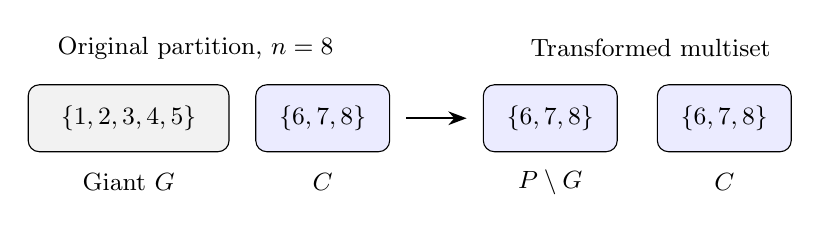
\begin{tikzpicture}[x=0.85cm,y=0.85cm,every node/.style={font=\small}]
  \node at (2.5,1.55) {Original partition, $n=8$};
  \draw[rounded corners,fill=black!5] (0,0) rectangle (3,1);
  \draw[rounded corners,fill=blue!8] (3.4,0) rectangle (5.4,1);
  \node at (1.5,0.5) {$\{1,2,3,4,5\}$};
  \node at (4.4,0.5) {$\{6,7,8\}$};
  \node at (1.5,-0.45) {Giant $G$};
  \node at (4.4,-0.45) {$C$};
  \draw[-{Stealth},thick] (5.65,0.5) -- (6.55,0.5);
  \node at (9.3,1.55) {Transformed multiset};
  \draw[rounded corners,fill=blue!8] (6.8,0) rectangle (8.8,1);
  \draw[rounded corners,fill=blue!8] (9.4,0) rectangle (11.4,1);
  \node at (7.8,0.5) {$\{6,7,8\}$};
  \node at (10.4,0.5) {$\{6,7,8\}$};
  \node at (7.8,-0.45) {$P\setminus G$};
  \node at (10.4,-0.45) {$C$};
\end{tikzpicture}
\caption{Replacing a giant cell by its complement can duplicate an
existing cell. Both occurrences are retained in every overlap sum.}
\label{fig:giant}
\end{figure}


This replacement removes the overlap of all pairs at very coarse
scales.  Its cost is a function of each endpoint separately, which
will disappear when pair laws with the same combined marginals are
compared.  Define
\begin{align*}
 M_j&=\sup\{r:G_j(r)\text{ exists}\},\\
 S_j(x)&=\int_{\{r:G_j(r)\text{ exists}\}}
              \1_{\{x\notin G_j(r)\}}\,dr,\\
 L_j(x,y)&=\int_\R\sum_{C\in\mathcal C_j(r)}
                    \1_C(x)\1_C(y)\,dr\qquad(x\ne y).
\end{align*}

\begin{lemma}\label{lem:hier-depth}
For each realized hierarchy on $n\ge2$ points, the displayed
quantities are finite and, for distinct $x,y$,
\begin{equation}\label{eq:depth}
 d_j(x,y)=M_j+L_j(x,y)-S_j(x)-S_j(y).
\end{equation}
They are integrable over the grids.  At every finite place where all
distinct coordinate differences are units, $M_j=S_j=L_j=0$.
\end{lemma}

\begin{proof}
Suppress $j$, and let $d_-$ and $d_+$ be the minimum and maximum of
the finitely many distinct-pair depths.  Below $d_-$ the partition
has only the cell $P$; above $d_+$ it has only singletons.  A giant
at any level has a giant ancestor at every coarser level.  Thus a
giant exists on an initial ray with endpoint $M\in[d_-,d_+]$,
up to an immaterial endpoint convention.

Let $o(r)=\1_{\{d(x,y)\ge r\}}$, $g(r)=\1_{\{G(r)\text{ exists}\}}$,
and $t(r)=\sum_{C\in\mathcal C(r)}\1_C(x)\1_C(y)$.  Expanding the
giant indicator through its complement gives the pointwise identity
\[
 o(r)-g(r)=t(r)
       -\1_{\{G(r)\text{ exists},\ x\notin G(r)\}}
       -\1_{\{G(r)\text{ exists},\ y\notin G(r)\}}.
\]
The integral of the left side is $d(x,y)-M$.  Each term on the
right vanishes outside $[d_-,d_+]$ on a distinct pair, and $t(r)\le2$.
Consequently integration proves~\eqref{eq:depth}, with bounds
\[
 0\le S(x)\le d_+-d_-,\quad
 0\le L(x,y)\le2(d_+-d_-),\quad
 |M|\le\max(|d_-|,|d_+|).
\]
These bounds are grid integrable by Lemma~\ref{lem:hier-grid}, since
the configuration has finitely many pairs and finite raw depths.
At a finite place with all raw depths zero, $d_-=d_+=0$, proving the final
assertion.  Ties change neither the identity nor any integral.
\end{proof}

The empty complement of $P$ and singleton occurrences contribute
zero to every distinct-pair overlap.  We do not define $L_j(x,x)$:
singleton cells persist to arbitrarily fine scales, so its integral
would be infinite.

\subsection{The exact overlap identity}

For a nonnegative or integrable quantity depending on the place
and grids, write
\[
 \avg{H}=\sum_v\sigma_v\E_{\mathrm{grids}}H,
 \qquad
 \I(g)=\avg{\sum_{j=1}^2\int_\R
                   \sum_{C\in\mathcal C_j(r)}g\,dr}.
\]
There is no grid randomness at finite places.  The integrand $g$
may also depend on the coordinate, level, and cell occurrence.
All sums over $\mathcal C_j(r)$ retain multiplicity.  These
notations do not assert finiteness for an arbitrary $g$; finiteness
will be established for each expression used.

Set
\[
 S^*(x)=\avg{S_1(x)+S_2(x)},\qquad
 L^*(x,y)=\avg{L_1(x,y)+L_2(x,y)}\quad(x\ne y).
\]
Lemma~\ref{lem:hier-depth} and the finite set of nonunit places show
that these quantities, and $\avg{M_1+M_2}$, are finite.  For each
distinct pair, the product formula and Lemma~\ref{lem:hier-grid}
give
\[
 \avg{d_1(x,y)+d_2(x,y)}=2\kappa.
\]
Taking expectations in~\eqref{eq:depth} is therefore legitimate and
yields the promised additive identity
\begin{equation}\label{eq:additive}
 L^*(x,y)=b_*+S^*(x)+S^*(y)\quad(x\ne y),
 \qquad b_*=2\kappa-\avg{M_1+M_2}.
\end{equation}
In particular, any signed law on distinct pairs with zero total
mass and zero sum of its two marginals has zero integral against
$L^*$.  This consequence is exact; no error from sampling a
diagonal pair is involved.

The three nonnegative finite scales used below are
\begin{equation}\label{eq:hier-scales}
 W_2=\I\bigl(\pi(C^2)\bigr)=\E_\pi L^*(x,y),\qquad
 A=\E_\alpha S^*(x),\qquad W=W_2+A.
\end{equation}
Thus $W_2$ measures distinct-pair overlap after the giant is
replaced, while $A$ measures the average time spent outside the
giant.  Equation~\eqref{eq:additive} relates these scales to the
graph and fiber laws.  Every absolute grid-error bound remains
uniform in $K$, since its archimedean weights sum to one.

\section{Small cells and fiber mass}\label{sec:smallcells}

We now combine the subset estimate with the overlap identity.  The goal is
to show that cells of size at most $n^{1-c}$ carry only $o(W+1)$ of the
off-diagonal overlap.  The main issue is a cell containing a source but
only a small fraction of its fiber; the paired coordinate will control
this contribution.

First, Equation~\eqref{eq:additive} and the uniform marginals of $\pi$
give $W_2=b_*+2A$.  If
$(q_X+q_Y)/2\ge(1-\epsilon_n)\alpha$, where $\epsilon_n\to0$, then
\[
 \E_q L^*(x,y)
 =W_2+\sum_{x\in P}
   \bigl(q_X(x)+q_Y(x)-2\alpha(x)\bigr)S^*(x).
\]
Since $S^*\ge0$ and $q\le B_0\pi$, it follows that
\begin{equation}\label{eq:q-overlap}
 W_2-o(1)A
 \le \I\bigl(q(C^2)\bigr)
 =\E_q L^*(x,y)
 \le B_0W_2.
\end{equation}
For a current cell occurrence $C$, write $a=\alpha(C)$ and
$p=\mu_e(C)$; the latter depends on the fiber $e$.  Define
\[
 T(\lambda)=\I\left(
   \E_e\1_C(x_e)p\,\1_{\{p<\lambda\}}\right).
\]
This is finite, since its integrand is at most
$q(C^2)=\E_e\1_C(x_e)\mu_e(C)$.

\begin{lemma}\label{lem:small-fiber}
For the prepared graph and its hierarchies, if
$0<\lambda<1/2$, $2/n\le\tau\le1$, and $H\ge1$, then
\begin{equation}\label{eq:small-fiber}
 T(\lambda)\ll
 \left(\frac{\lambda}{\tau^2}+\lambda\right)W_2
 +\tau A+\lambda H+e^{-b_1H},
\end{equation}
where $b_1>0$ is absolute.  The implicit constant depends only on $B_0$
and the absolute constants in Equation~\eqref{eq:grid-error}.
\end{lemma}

\begin{proof}
We separate large cells, complements of giants, and actual small cells.
For a set of size $m\ge2$,
\begin{equation}\label{eq:sc-pair-comparison}
 \frac{\alpha(C)^2}{2}
 \le \pi(C^2)=\frac{m(m-1)}{n(n-1)}
 \le\alpha(C)^2.
\end{equation}
If $a\ge\tau$, then $m\ge2$ and the integrand of $T(\lambda)$ is
at most $\lambda\le2\lambda\pi(C^2)/\tau^2$.  These occurrences
contribute at most $2\lambda W_2/\tau^2$.
If $C$ is the complement occurrence of a giant and $a<\tau$, its
contribution is at most
\[
 q(C^2)\le B_0\pi(C^2)\le B_0\tau a.
\]
The integral of $a$ over the giant-complement occurrences is $A$,
so their contribution is at most $B_0\tau A$.
These two classes retain the multiplicities of the transformed family.

It remains to treat actual nongiant cells of mass less than $\tau$.
Fix a place, a coordinate $j$, and the two entire realized hierarchies.
Let $j'$ be the other coordinate and set $H_v=H$ at archimedean places,
$H_v=0$ otherwise.  For a fiber $e$ with source $x=x_e$, let $U$
be the actual $j$-cell containing $x$ at level $r$, and put
$p=\mu_e(U)$.  We retain only the levels with $U$ nongiant,
$\alpha(U)<\tau$, and $p<\lambda$.
Without grid errors, a fiber point outside the source cell in coordinate
$j$ lies inside the source cell at the complementary level $h_e-r$ in
coordinate $j'$.  We use two nearby levels in the latter coordinate to
measure failures of this complementarity.  Define the cells
\[
 V_-=\Pi_{j'}(h_e-r-H_v)(x),\qquad
 V_+=\Pi_{j'}(h_e-r+H_v)(x),
\]
where $\Pi_j(t)(x)$ denotes the cell of $x$ in $\Pi_j(t)$.
Thus $V_+\subseteq V_-$.  The two errors are
\[
 D^-=\mu_e\bigl(P\setminus(U\cup V_-)\bigr),\qquad
 D^+=\mu_e(U\cap V_+).
\]

The fiber identity makes these errors small after integration.  For a
fixed fiber point $y$, write $d=d_j(x,y)$ and $d'=d_{j'}(x,y)$.
Its contribution to $D^-$ occurs when
$d<r<h_e-H_v-d'$, and its contribution to $D^+$ occurs when
$h_e+H_v-d'\le r\le d$.  Hence
\begin{align*}
 \int D^-\,dr&=\E_{y\sim\mu_e}(h_e-d-d'-H_v)_+,\\
 \int D^+\,dr&=\E_{y\sim\mu_e}(d+d'-h_e-H_v)_+.
\end{align*}
Their sum is the expectation of
$(|\Delta_j(x,y)+\Delta_{j'}(x,y)|-H_v)_+$, since
$i_j(x,y)+i_{j'}(x,y)=h_e$.  At nonarchimedean places it is zero.
At archimedean places Equation~\eqref{eq:grid-error} and the union bound
give
\[
 \Pr\bigl(|\Delta_j+\Delta_{j'}|>u\bigr)
 \le2C_0e^{-b_0u/2}.
\]
Integrating this tail, averaging over fibers, and using
$\sum_{v\mid\infty}\sigma_v=1$, we obtain
\begin{equation}\label{eq:sc-errors}
 \avg{\E_e\int(D^-+D^+)\,dr}\ll e^{-b_1H}.
\end{equation}
No independence of the two errors is required.

We now split the retained levels into three cases.  In each change of
level below the fiber is fixed, so $h_e$ is constant; both realized
hierarchies are held fixed over all levels before any averaging.

\smallskip\noindent
\emph{Case 1: $V_-$ is nongiant.}
Since $\mu_e(V_-)+D^-\ge1-p>1/2$,
\[
 p\le2\lambda\bigl(\mu_e(V_-)+D^-\bigr).
\]
After discarding the other restrictions, change levels to
$r'=h_e-r-H_v$.  Sharing a nongiant cell in the $j'$-hierarchy
contributes to $L_{j'}$, so the main term is bounded by
$2\lambda\E_qL_{j'}$.  Summing over coordinates and places gives
at most $2B_0\lambda W_2$.  The error is bounded by
Equation~\eqref{eq:sc-errors}, since $2\lambda<1$.

\smallskip\noindent
\emph{Case 2: $V_-$ is giant and $V_+$ is not.}
For a fixed source $x$, the levels at which its cell in the
$j'$-hierarchy is giant form an initial interval, by nesting.
The two levels defining $V_-$ and $V_+$ straddle its endpoint, so
the allowed $r$ have length at most $2H_v$.  As $p<\lambda$, this
costs at most $2\lambda H_v$ per fiber.  Summing and averaging gives
at most $4\lambda H$.

\smallskip\noindent
\emph{Case 3: $V_+$ is giant.}
This is the remaining case, since $V_+\subseteq V_-$.  Here
\[
 p=D^++\mu_e(U\setminus V_+).
\]
The first term is covered by Equation~\eqref{eq:sc-errors}.
In the second change levels to $r'=h_e-r+H_v$ for each fiber.
At a fixed new level, every counted pair has
$y\notin G_{j'}(r')$ and shares an actual $j$-cell of size less than
$\tau n$ at some original level.

For a fixed target $y$, let $N_j(y)$ be the union of all actual
$j$-cells containing $y$ whose size is less than $\tau n$, over all
levels.  These cells form a nested chain of subsets of the finite set
$P$, so $|N_j(y)|<\tau n$ (with empty union allowed).
Thus all the possible sources of this target lie in
$N_j(y)\setminus\{y\}$, even though their selected levels depend on
the fiber.  Each edge belongs to exactly one fiber and retains weight
$1/|E|$ after the level change.  The mass at $r'$ is therefore at most
\begin{align*}
 &\sum_{y\notin G_{j'}(r')}
   \sum_{x\in N_j(y)\setminus\{y\}}q(x,y)\\
 &\hspace{1cm}\le
 \frac{B_0}{n(n-1)}
 \sum_{\substack{y\notin G_{j'}(r')\\N_j(y)\ne\varnothing}}
       (|N_j(y)|-1)
 \le B_0\tau\alpha\bigl(P\setminus G_{j'}(r')\bigr).
\end{align*}
In the last step, $|N_j(y)|-1\le\tau(n-1)$ because $\tau\le1$.
Integrating, summing coordinates and averaging gives $B_0\tau A$.

The three cases, the initial split, and Equation~\eqref{eq:sc-errors}
prove Equation~\eqref{eq:small-fiber}.  Threshold ties affect only
endpoints of level intervals.  All rearranged integrands are
nonnegative, so Tonelli's theorem applies.
\end{proof}

We can now discard the small cells in the overlap scale.  Recall
$\lambda_n=1/\log n$.  Taking
$\tau=\lambda_n^{1/3}$ and $H=\lambda_n^{-1/2}$ in
Lemma~\ref{lem:small-fiber} gives
\[
 T(\lambda_n)
 \ll\lambda_n^{1/3}W+\lambda_n^{1/2}
       +e^{-b_1\lambda_n^{-1/2}}
 =o(W+1).
\]
Define
\[
 W_{2,\mathrm{sm}}=
 \I\bigl(\pi(C^2)\1_{\{|C|\le n^{1-c}\}}\bigr).
\]
Split $\I(q(C^2))$ according to whether
$\mu_e(C)<\lambda_n$.  Equation~\eqref{eq:subset}, whose errors are
uniform in every subset $C$, bounds the other part by
\[
 (1+o(1))(W_2-W_{2,\mathrm{sm}})+o(1)W_{2,\mathrm{sm}}.
\]
Adding $T(\lambda_n)=o(W+1)$ and comparing with
Equation~\eqref{eq:q-overlap} yields
\begin{equation}\label{eq:small-overlap}
 W_{2,\mathrm{sm}}=o(W+1).
\end{equation}
This estimate holds before passing to either a bounded or an unbounded
subsequence of $W$.

\section{Variance from off-diagonal sampling}\label{sec:variance}

We now use the additive overlap identity to compare the mass of a cell
under a fiber law with its mass under the uniform law.  The same argument
will apply to the conditional law of sources arriving at a target.  It
is essential to sample distinct pairs throughout: the hierarchy has an
infinite range of singleton levels, so a small diagonal error cannot be
integrated indiscriminately.

\begin{lemma}\label{lem:variance}
Let $\mathcal F$ be a finite family of probability measures $\nu$, each
uniform on a subset $B\subset P$ of size $k\ge n^\gamma$.  Give the family
nonnegative weights, independent of places and grids, of total mass at
most one, and write $\E_{\mathcal F}$ for the weighted sum.  Suppose
$\E_{\mathcal F}\nu\le M\alpha$ pointwise, where $M$ is fixed.
For each transformed cell occurrence $C$, put
$m=|C|$, $a=\alpha(C)$, and $p=\nu(C)$.  Then
\begin{align}
\I\!\left(\E_{\mathcal F}\left[
  (p-a)^2\1_{\{m>n^{1-c}\}}
  +p^2\1_{\{m\le n^{1-c},\ p\ge2/k\}}
\right]\right)
&\le C_M\bigl(n^{c-\gamma}W_2+W_{2,\mathrm{sm}}\bigr)
\label{eq:variance-quant}\\
&=o(W+1).
\label{eq:variance}
\end{align}
The constant $C_M$ depends only on $M$.
\end{lemma}

The first term measures discrepancy from $\alpha$ on cells large enough
for the finite-population corrections to be negligible.  On a small
cell, the second term measures $\nu$-mass only when $B\cap C$ contains
at least two points: a one-point intersection contributes no
distinct-pair overlap within $B$.

\begin{proof}
The proof uses an exact signed identity for pair probabilities, followed
by separate estimates on large cells, small cells, and singletons.
The integer $k\ge n^\gamma>1$ is at least two.  Let $P_B$ be the uniform
law on distinct ordered pairs from $B$.  Define another law $R_B$ on
distinct pairs as follows.  First take $X$ uniformly from $B$.  If $k<n$,
then, conditionally on $X$, take $Y$ uniformly from $B\setminus\{X\}$
with probability $k/n$, and uniformly from $P\setminus B$ otherwise.
If $B=P$, define $R_B=P_B=\pi$ directly; the outside branch has zero
probability and need not be defined.

The first marginal of $R_B$ is $\nu$, and its second marginal is exactly
$\alpha$.  Indeed, a point $y\in B$ receives mass
\[
 (k-1)\frac1k\frac{k}{n}\frac1{k-1}=\frac1n,
\]
and a point $y\notin B$ receives mass
$k(1/k)((n-k)/n)/(n-k)=1/n$.  Thus the signed measure
$P_B-2R_B+\pi$ has total mass zero.  Its first and second marginals are
$\alpha-\nu$ and $\nu-\alpha$, respectively, so their sum is zero.
The additive overlap identity~\eqref{eq:additive} gives
\begin{equation}\label{eq:variance-cancel}
 \I\bigl(P_B(C^2)-2R_B(C^2)+\pi(C^2)\bigr)=0.
\end{equation}
This identity involves finite integrals.  For fixed $n$, any probability
law on distinct pairs is bounded by $n(n-1)\pi$ pointwise, so each of the
three nonnegative terms has a finite integral because $W_2<\infty$.
The family weights are independent of places and grids; hence we may
average~\eqref{eq:variance-cancel} over the family.

We calculate the three cell probabilities before making any estimates.
Writing $b=|B\cap C|$, so that $p=b/k$, gives
\begin{align*}
 P_B(C^2)
 &=\frac{b(b-1)}{k(k-1)}
   =p^2-\frac{p(1-p)}{k-1},\\
 R_B(C^2)
 &=p\left(\frac{k}{n}\frac{b-1}{k-1}+\frac{m-b}{n}\right)
   =ap-\frac{k}{n}\frac{p(1-p)}{k-1},\\
 \pi(C^2)
 &=\frac{m(m-1)}{n(n-1)}
   =a^2-\frac{a(1-a)}{n-1}.
\end{align*}
The middle identity also holds when $k=n$, by the direct definition of
$R_B$.  Therefore, with
$H_B(C)=P_B(C^2)-2R_B(C^2)+\pi(C^2)$,
\begin{equation}\label{eq:variance-finite}
 H_B(C)=(p-a)^2+\left(\frac{2k}{n}-1\right)
                 \frac{p(1-p)}{k-1}
                 -\frac{a(1-a)}{n-1}.
\end{equation}
Write $\overline H=\E_{\mathcal F}H_B$ and
$\omega=\E_{\mathcal F}1\le1$.  In the averaged formula, the last term
in~\eqref{eq:variance-finite} is multiplied by $\omega$.

First suppose $m>n^{1-c}$.  Since
$1/(k-1)\le2n^{-\gamma}$, $1/(n-1)\le2n^{-\gamma}$, and
$\E_{\mathcal F}p\le Ma$, Equation~\eqref{eq:variance-finite} implies
\[
 \overline H(C)\ge\E_{\mathcal F}(p-a)^2
                   -2(M+1)n^{-\gamma}a.
\]
For every $m\ge2$ we have
\begin{equation}\label{eq:variance-pair-comparison}
 \tfrac12a^2\le\pi(C^2)\le a^2.
\end{equation}
Here $a>n^{-c}$, so
$n^{-\gamma}a\le2n^{c-\gamma}\pi(C^2)$.  Hence
\begin{equation}\label{eq:variance-large}
 \overline H(C)\ge\E_{\mathcal F}(p-a)^2
       -4(M+1)n^{c-\gamma}\pi(C^2).
\end{equation}

Next suppose $2\le m\le n^{1-c}$.  If $p\ge2/k$, then $b\ge2$ and
\[
 P_B(C^2)=p^2\frac{k}{k-1}\frac{b-1}{b}\ge\tfrac12p^2.
\]
Since $P_B(C^2)$ is always nonnegative, this proves
$P_B(C^2)\ge\tfrac12p^2\1_{\{p\ge2/k\}}$ for every $B$.
Also $R_B(C^2)\le ap$, and therefore
\[
 \E_{\mathcal F}R_B(C^2)\le Ma^2\le2M\pi(C^2).
\]
Discarding the nonnegative term $\omega\pi(C^2)$ yields
\begin{equation}\label{eq:variance-small}
 \overline H(C)\ge\tfrac12\E_{\mathcal F}
                \bigl[p^2\1_{\{p\ge2/k\}}\bigr]-4M\pi(C^2).
\end{equation}

Finally, if $m=0$ or $m=1$, all three pair probabilities vanish exactly.
For a singleton, $p$ is either zero or $1/k$, so the small-cell term in
the conclusion vanishes too; a singleton cannot satisfy
$m>n^{1-c}$.  This exact cancellation treats the infinite singleton
tails.  We never integrate the separate correction terms
in~\eqref{eq:variance-finite} over those tails.

Integrate~\eqref{eq:variance-large} and~\eqref{eq:variance-small} on
their respective regions, use the exact zero on empty and singleton
cells, and apply~\eqref{eq:variance-cancel}.  The result is
\begin{align*}
 \I\!\left(\E_{\mathcal F}\left[
 (p-a)^2\1_{\{m>n^{1-c}\}}
 +\tfrac12p^2\1_{\{m\le n^{1-c},\ p\ge2/k\}}
 \right]\right)
 \le 4(M+1)n^{c-\gamma}W_2+4M W_{2,\mathrm{sm}}.
\end{align*}
The nonnegative left-hand terms are integrable by these pointwise
bounds and the integrability of $\overline H$ and the displayed errors.
Doubling the bound proves~\eqref{eq:variance-quant}, with
$C_M=8(M+1)$.

All the cell estimates hold for arbitrary subsets of $P$.
They therefore include giant complements and count repeated cell
occurrences with their original multiplicity.  In the special case
$B=P$, the signed expression and the large-cell variance are zero;
the small-cell term may equal $a^2$, which is absorbed by
$2\pi(C^2)$ as above.  Finally, $c<\gamma$, $W_2\le W$, and
Equation~\eqref{eq:small-overlap} give~\eqref{eq:variance}.
\end{proof}

We will use Lemma~\ref{lem:variance} for two families.  For the fiber
laws $\mu_e$, with weights $k_e/|E|$, the weights sum to one and
\[
 \E_e\mu_e=q_Y\le B_0\alpha.
\]
Their support sizes satisfy $k_e\ge n^{s-o(1)}\ge n^\gamma$ for all
sufficiently large $n$, since $\gamma<s$.

For the incoming laws $\rho_y$, retain the targets whose incoming
degree $d_y$ is at least $n^\gamma$, and use weights
$q_Y(y)=d_y/|E|$.  Their weighted mean is dominated by $q_X$:
\[
 \sum_{y:d_y\ge n^\gamma}q_Y(y)\rho_y\le q_X\le B_0\alpha.
\]
Each retained law is uniform on its $d_y$ incoming sources, and the
family weights have total mass at most one.  Both families are defined
by the same finite graph at every place, as required by the lemma.
The omitted targets have total mass
\begin{equation}\label{eq:variance-omitted}
 \sum_{y:d_y<n^\gamma}q_Y(y)
 \le\frac{n^{1+\gamma}}{|E|}
 =O(n^{\gamma-1})=o(1),
\end{equation}
because the edge density tends to $\theta>0$ and $\gamma<1$.
Thus the cell-mass estimates apply both to outgoing fibers and to
almost all incoming conditional laws.  These are the two distributions
that the remaining argument must compare with $\alpha$.

\section{The case of unbounded overlap scale}\label{sec:unbounded}

The scale $W=W_2+A$ is finite and nonnegative for each configuration.
Every counterexample sequence therefore has a bounded-$W$ subsequence
or a subsequence on which $W\to\infty$. We treat the latter here;
Section~\ref{sec:bounded} treats the bounded alternative.
Suppose, then, that $W\to\infty$. We will derive a
contradiction from the variance estimate and the equation defining each
fiber. First we show that a positive fraction of $W$ comes from cells
whose uniform masses stay away from zero. These cells define finite
weighted trees. Transport on the trees will turn the fiber equation into
an impossible assertion about three independent uniform vertices.
Throughout this section, $o(W+1)=o(W)$.

\subsection{Extracting cells of positive mass}

We first claim that
\begin{equation}\label{eq:unb-overlap-scale}
 W_2\ge c_1 W
\end{equation}
for some fixed $c_1>0$ and all sufficiently large $n$. At a fixed
place and choice of grids, abbreviate $S=S_1+S_2$ and $L=L_1+L_2$.
Choose a fiber $e$ with its edge-induced weight and then choose $Y,Y'$
independently with law $\mu_e$. Equation~\eqref{eq:depth} and the
constant raw depth sum on the fiber give
\[
 S(Y)=M_1+M_2-S(x_e)-h_e+L(x_e,Y)
       -\Delta_1(x_e,Y)-\Delta_2(x_e,Y).
\]
All source--neighbor pairs are distinct. Thus the first-moment bound
from~\eqref{eq:grid-error}, the normalization of the archimedean
weights, and~\eqref{eq:q-overlap} imply
\[
 \avg{\E|S(Y)-S(Y')|}\le 2\avg{\E_q L(x,y)}+O(1)
 =O(W_2)+O(1).
\]
To compare this with $A$, we use the pointwise bound
\begin{equation}\label{eq:potential}
 S^*(x)\ge A-2W_2\qquad(n>2).
\end{equation}
Indeed, the average of $L^*(x,y)$ over the $n-1$ labels $y\ne x$ equals
\[
 W_2+\frac{n-2}{n-1}\bigl(S^*(x)-A\bigr),
\]
and is nonnegative.  Hence $\avg{\E S(Y)}\ge A-2W_2$.
Consequently
\begin{equation}\label{eq:unb-min-lower}
 \avg{\E\min\{S(Y),S(Y')\}}\ge A-O(W_2)-O(1).
\end{equation}

For two nonnegative lists $(a_1,a_2)$ and $(b_1,b_2)$,
\[
 \min\{a_1+a_2,b_1+b_2\}\le\sum_{i,j=1}^2\min\{a_i,b_j\}.
\]
Indeed, if the first sum is smaller, then
$\sum_j\min\{a_i,b_j\}\ge a_i$ for each $i$. Moreover, nesting of the
giants gives, for almost every $u>0$,
\[
 \{z:S_i(z)>u\}=P\setminus G_i(M_i-u).
\]
A vertex which leaves the giant at level $r_z<M_i$ has
$S_i(z)=M_i-r_z$; one which never leaves has $S_i(z)=0$. This proves
the displayed identity, with only finitely many possible threshold ties.
Conditional independence of $Y,Y'$ and $ab\le(a^2+b^2)/2$ now give
\begin{equation}\label{eq:unb-min-upper}
 \avg{\E\min\{S(Y),S(Y')\}}
 \le 2\avg{\sum_{i=1}^2\E_e\int_{r<M_i}
          \mu_e(P\setminus G_i(r))^2\,dr}.
\end{equation}
To bound the right side, write $p=\mu_e(C)$ and $a=\alpha(C)$ for a
giant-complement occurrence. If $|C|>n^{1-c}$, use
$p^2\le2(p-a)^2+2a^2$, the variance estimate~\eqref{eq:variance}, and
$a^2\le2\pi(C^2)$. For smaller complements with $p\ge2/k_e$, use
the second term of~\eqref{eq:variance}. The remaining terms satisfy
$p^2\le2n^{-\gamma}p$. Since $\E_e p=q_Y(C)\le B_0a$, their integral
is $O(n^{-\gamma}A)$. In particular, this last error is charged to
$A$, the finite integral of the complement masses. We obtain
\[
 \avg{\E\min\{S(Y),S(Y')\}}
 \le O(W_2)+o(W)+O(n^{-\gamma}A).
\]
Together with~\eqref{eq:unb-min-lower}, this proves
$A\le O(W_2)+o(W)+O(1)$, and hence~\eqref{eq:unb-overlap-scale}.
Equation~\eqref{eq:q-overlap} also gives $\I(q(C^2))\gg W$.

We next restrict the masses of the cells we use. For a fixed
$0<\delta<1/4$, split the contribution of $a\le\delta$ according to
$p<2\delta$ or $p\ge2\delta$. In the latter case
$p\le p^2/(2\delta)$ and $p-a\ge p/2$. On large cells this is
controlled by the first variance term; on small cells,
$p\ge2\delta\ge2/k_e$ eventually, so the second variance term applies.
Therefore
\[
 \I\bigl(\1_{\{a\le\delta\}}q(C^2)\bigr)
 \le T(2\delta)+o_\delta(W)
 \le O(\delta^{1/3}W)+o_\delta(W).
\]
For the last inequality apply Lemma~\ref{lem:small-fiber} with
$\lambda=2\delta$, $\tau=\lambda^{1/3}$ and any fixed $H\ge1$.
The terms depending only on $\delta,H$ are $o_\delta(W)$.
The implicit constant in $O(\delta^{1/3}W)$ is independent of $\delta$.
We may thus choose $\delta$ sufficiently small once and for all, and
then let $n\to\infty$, to obtain
\begin{equation}\label{eq:cut-mass}
 \I(\1_{\{a>\delta\}})\gg W,
 \qquad
 \I(\1_{\{a\ge\delta/4\}})\ll_\delta W.
\end{equation}
The first inequality uses $q(C^2)\le1$. For the second, when $n$ is
large, $a\ge\delta/4$ implies
$\pi(C^2)\ge a^2/2\ge\delta^2/32$.
All cutoffs below use this fixed $\delta$; in particular, a bound
$O_\delta(1)$ is $o(W)$ along the present subsequence.

Choose a Lipschitz function $w:[0,1]\to[0,1]$ satisfying
\[
 w(u)=w(1-u),\qquad
 w=0\text{ on }[0,\delta/2]\cup[1-\delta/2,1],\qquad
 w=1\text{ on }[\delta,1-\delta].
\]
For the original partitions, define
\[
 \ell_j=\int_{\R}\sum_{B\in\Pi_j(r)}w(\alpha(B))\,dr.
\]
Replacing a giant by its complement preserves every summand by
symmetry, with occurrences still counted separately. Thus
\begin{equation}\label{eq:unb-total-length}
 W\ll\avg{\ell_1+\ell_2}\ll_\delta W.
\end{equation}

For either family of measures in Lemma~\ref{lem:variance}, we shall use
\begin{equation}\label{eq:cut-approx}
 \avg{\E_{\mathcal F}\sum_{j=1}^2\int_{\R}
 \sum_{B\in\Pi_j(r)}
 \left[|w(\nu(B))-w(\alpha(B))|
       +w(\alpha(B))|\nu(B)-\alpha(B)|\right]dr}=o(W).
\end{equation}
The first term lets us replace cut weights defined by the fiber laws
with those defined by the uniform law.  The second controls the weighted
mass imbalance that will appear in the transport comparison.
Here the family of incoming laws retains only targets with at least
$n^\gamma$ incoming neighbors, as in Section~\ref{sec:variance}.
To prove~\eqref{eq:cut-approx}, note first that its integrand is
unchanged under $(p,a)\mapsto(1-p,1-a)$. Work therefore with the
transformed cells. On $a\ge\delta/4$, all cells are large for large
$n$; the Lipschitz bound, Cauchy--Schwarz,
\eqref{eq:cut-mass}, and~\eqref{eq:variance} give $o(W)$.
On $a<\delta/4$, the second summand vanishes, and the first can be
nonzero only if $p>\delta/2$. For large cells,
$1\le16\delta^{-2}(p-a)^2$; for small cells,
$1\le4\delta^{-2}p^2$ and $p\ge2/k$ eventually. The same variance
estimate again gives $o(W)$.

\subsection{Distances obtained from the hierarchy}

We have retained a positive total amount of cells, and the masses of
those cells are close to their $\alpha$-masses in the fiber average. We now use these cells as cuts defining a distance. For
$\nu=\alpha$ or $\mu_e$, put
\[
 D_j^\nu(a_0,a_1)=\int_{\R}\sum_{B\in\Pi_j(r)}
 |\1_B(a_0)-\1_B(a_1)|\,w(\nu(B))\,dr.
\]
We also allow a formal endpoint $\infty$, setting $\1_B(\infty)=0$
for every cell. These quantities are finite for all sufficiently large
$n$. On the initial ray the only cell is $P$, of weight $w(1)=0$;
on the final ray all cells are singletons, of $\nu$-mass either
$0$, $1/n$, or $1/k_e$, so their weights vanish too.

For distinct $a_0,a_1\in P$ we have
\begin{equation}\label{eq:projection}
 D_j^\nu(a_0,a_1)=\int_{\R}
 w\bigl(\nu\{z:d_j(a_1,z)-d_j(a_0,z)\ge u\}\bigr)\,du.
\end{equation}
Indeed, set $d_0=d_j(a_0,a_1)$. Nestedness implies that if
$d_j(a_1,z)>d_0$, then $d_j(a_0,z)=d_0$, and conversely with the
indices exchanged. Otherwise the two depths to $z$ agree.
For $u>0$ the event in~\eqref{eq:projection} is the $a_1$-cell at
level $d_0+u$. For $u<0$ its complement is the $a_0$-cell at level
$d_0-u$, up to strict versus weak threshold ties. There are only
finitely many finite depths, so those ties have zero Lebesgue measure.
Splitting the integral at zero and using $w(t)=w(1-t)$ gives exactly
the two cell contributions above their common depth $d_0$.
The depth difference is $+\infty$ at $z=a_1$ and $-\infty$ at
$z=a_0$; no difference $\infty-\infty$ occurs. Directly from the
cell definition, we also have
\begin{equation}\label{eq:unb-root-projection}
 D_j^\nu(\infty,y)=\int_{\R}
 w\bigl(\nu\{z:d_j(y,z)\ge u\}\bigr)\,du.
\end{equation}

For an edge $(x,y)$ in fiber $e$, put $j'=3-j$. The fiber equation
implies, for $z\in F_e$,
\[
 Z_{j'}(z)=Z_{j'}(x)+\frac{t_e}{Z_j(z)-Z_j(x)}.
\]
Consequently, for $z\ne y$ in this fiber,
\[
 Z_{j'}(z)-Z_{j'}(y)
 =\frac{t_e\bigl(Z_j(y)-Z_j(z)\bigr)}
 {(Z_j(z)-Z_j(x))(Z_j(y)-Z_j(x))},
\]
and hence
\begin{equation}\label{eq:unb-raw-fiber}
 i_{j'}(y,z)=i_j(y,z)-i_j(x,z)+h_e-i_j(x,y).
\end{equation}
This identity converts one of the projected distances into a root
distance in the other coordinate. Here are the details, including the
diagonal atom. Under $z\sim\mu_e$, compare
\[
 U(z)=d_{j'}(y,z),\qquad
 V(z)=d_j(y,z)-d_j(x,z)+h_e-i_j(x,y).
\]
For $z\ne y$, Equation~\eqref{eq:unb-raw-fiber} gives
\[
 |U(z)-V(z)|\le
 |\Delta_{j'}(y,z)|+|\Delta_j(y,z)|+|\Delta_j(x,z)|.
\]
At $z=y$, both variables are $+\infty$, so their indicators at every
finite threshold agree; $z=x$ has zero $\mu_e$-mass. Tonelli's theorem
therefore gives the precise bound
\[
 \int_{\R}|\Pr(U\ge u)-\Pr(V\ge u)|\,du
 \le \sum_{z\in F_e\setminus\{y\}}\mu_e(z)|U(z)-V(z)|.
\]
Translation of the threshold by $h_e-i_j(x,y)$ does not change the
integral of the weighted tail. Apply the Lipschitz bound for $w$,
\eqref{eq:projection}, and~\eqref{eq:unb-root-projection}. After
averaging over $e$, $y\sim\mu_e$, grids and places, we obtain
\[
 \avg{\E_q
 |D_j^{\mu_e}(x,y)-D_{j'}^{\mu_e}(\infty,y)|}=O_\delta(1).
\]
The error estimate is valid for these sampling laws because
\eqref{eq:grid-error} bounds the grid first moment uniformly for
every distinct pair. All vertex laws are independent of the grids;
nonarchimedean errors vanish and the archimedean weights sum to one.

Changing $\mu_e$ to $\alpha$ changes any one of its cut distances by
at most $\int\sum_B|w(\mu_e(B))-w(\alpha(B))|\,dr$, independently
of the endpoints. Thus~\eqref{eq:cut-approx}, with
$D_j=D_j^\alpha$, yields
\begin{equation}\label{eq:fiber-tree}
 \avg{\E_q|D_j(x,y)-D_{j'}(\infty,y)|}=o(W).
\end{equation}
The remaining task is to replace the edge law in this equation by
independent uniform vertices and then exploit the geometry of the
cut distances.

\subsection{Transport to independent uniform vertices}

Each $D_j$ is the path distance on a finite weighted tree, allowing
zero-length edges. To see this, take the distinct cells of the nested
partitions as vertices, root the inclusion tree at $P$, and connect
each proper cell $B$ to its least strict supercell. Give this edge
length
\[
 l_j(B)=\int_{\R}\1_{\{B\in\Pi_j(r)\}}w(\alpha(B))\,dr.
\]
The points of $P$ are singleton leaves. An edge is crossed by their
connecting path exactly when its cell separates them, proving the
cut formula for $D_j$. The total edge length is exactly $\ell_j$.
The formal endpoint is represented by the root, since the root-cell
weight is zero.

For probabilities $\rho,\alpha$ on the leaves, let
$\mathsf T_j(\rho,\alpha)$ be the least expected $D_j$-distance among
couplings of the two laws. The tree transport formula is
\begin{equation}\label{eq:unb-transport}
 \mathsf T_j(\rho,\alpha)
 =\sum_{B\ne P}l_j(B)|\rho(B)-\alpha(B)|
 =\int_{\R}\sum_{B\in\Pi_j(r)}
       w(\alpha(B))|\rho(B)-\alpha(B)|\,dr.
\end{equation}
This standard formula is the finite-tree form of
\cite[Section~2, Equation~(5)]{TreeTransport}. It has a
short direct proof. Across the edge above $B$, any coupling must move
at least $|\rho(B)-\alpha(B)|$ units of mass. Conversely, first match
common mass at each leaf. Work upward, matching surplus mass from child
subtrees to deficits in other child subtrees, and send only the
remaining imbalance toward the parent. Across each edge the total
mass moved is precisely its absolute imbalance; the root imbalance
is zero. Decomposing these finitely many transfers into leaf-to-leaf
paths gives a coupling attaining the displayed cost. Zero-length
edges do not affect the argument.

By $q_Y=\E_e\mu_e$, convexity and~\eqref{eq:cut-approx} give
\begin{equation}\label{eq:unb-two-costs}
 \avg{\mathsf T_j(q_Y,\alpha)}=o(W),\qquad
 \avg{\E_{q_Y}\mathsf T_j(\rho_y,\alpha)}=o(W).
\end{equation}
For the second estimate, first apply~\eqref{eq:cut-approx} to targets
with at least $n^\gamma$ incoming neighbors. The omitted $q_Y$-mass
is $O(n^{\gamma-1})=o(1)$, independent of the hierarchy. Every
transport cost is at most $\ell_j$, so its omitted contribution is
$o(1)\avg{\ell_j}=o(W)$ by~\eqref{eq:unb-total-length}.

The conditional source law in Equation~\eqref{eq:fiber-tree}, given
the target $y$, is $\rho_y$. We keep this conditioning while coupling
the sources to the uniform law.
Fix a hierarchy for a moment and put
$F(x,x',y)=|D_j(x,y)-D_j(x',y)|$. If $Y\sim q_Y$ and $X,X'$ are
independent with conditional law $\rho_Y$, then
\[
 \E F(X,X',Y)
 \le2\E_q|D_j(x,y)-D_{j'}(\infty,y)|.
\]
For each $y$, use two independent copies of an optimal coupling of $\rho_y$
to $\alpha$, replacing $X,X'$ by $U,U'$. Conditional on $y$, the
new points are independent with law $\alpha$; since that law does
not depend on $y$, they are also independent of $Y$. The triangle
inequality bounds the change in $F$ by the sum of the two transport
distances. Next optimally couple $Y\sim q_Y$ to $V\sim\alpha$, independently
of $U,U'$. Moving the last argument of $F$ costs at most twice its
transport distance. We have proved the pointwise inequality
\begin{align*}
 \E_{\alpha^{\otimes3}}F
 &\le 2\E_q|D_j(x,y)-D_{j'}(\infty,y)|\\
 &\quad+2\E_{q_Y}\mathsf T_j(\rho_y,\alpha)
       +2\mathsf T_j(q_Y,\alpha).
\end{align*}
Its right side consists of explicit finite cut sums, so no selection
of couplings across places or random grids is required. Integrating
and using~\eqref{eq:fiber-tree} and~\eqref{eq:unb-two-costs} gives
\begin{equation}\label{eq:iid-tree}
 \avg{\E_{x,x',y\ \mathrm{iid}\ \alpha}
 |D_j(x,y)-D_j(x',y)|}=o(W).
\end{equation}

\subsection{A lower bound for tree distance fluctuations}

We finish with an elementary fact whose constants do not depend on
the shape of the tree.

\begin{lemma}\label{lem:unb-tree-fluctuation}
Let a finite tree have nonnegative edge lengths of total sum $L$,
with path pseudometric $d$, and let $\alpha$ be a probability on its
vertices. Suppose every edge of
positive length separates two sets each having $\alpha$-mass at least
$\delta/2$, where $0<\delta<1$. If $X,X',Y$ are independent with
law $\alpha$, then
\[
 \E|d(X,Y)-d(X',Y)|\ge
 \frac{\delta^2}{32(\lceil16/\delta\rceil+1)}L.
\]
\end{lemma}

\begin{proof}
There is nothing to prove if $L=0$. For every fixed $y$, the expected
distance from $X$ to $y$ is at least $\delta L/2$: each positive
edge separates $y$ from mass at least $\delta/2$. Since all distances
are at most $L$,
\[
 \Pr\{d(X,y)\ge\delta L/4\}\ge\delta/4.
\]
Traverse the tree in a closed walk crossing each edge twice, of total
length $2L$. Partition this walk into at most
$M=\lceil16/\delta\rceil+1$ intervals of length at most $\delta L/8$,
and assign each vertex to an interval containing one chosen visit.
The resulting classes have diameter at most $\delta L/8$. Thus
\[
 \Pr\{d(X',Y)\le\delta L/8\}
 \ge\sum_{r=1}^M\alpha(C_r)^2\ge1/M.
\]
Conditional on $Y$, the far event for $X$ and the near event for $X'$
are independent. The far probability is uniformly at least $\delta/4$,
so both events occur with probability at least $\delta/(4M)$.
On their intersection the absolute difference of the distances is
at least $\delta L/8$, proving the claim.
\end{proof}

In the tree for $D_j$, every positive edge has both side masses greater
than $\delta/2$, by the support condition on $w$. Apply
Lemma~\ref{lem:unb-tree-fluctuation} with $L=\ell_j$, sum over
$j=1,2$, and average over places and grids. Equations
\eqref{eq:unb-total-length} and~\eqref{eq:iid-tree} give
$W\ll o(W)$, a contradiction. This excludes every subsequence on
which $W\to\infty$.

\section{Bounded scale and a limiting fiber map}\label{sec:bounded}

It remains to exclude a subsequence on which $W$ is bounded.
We will choose one complex embedding and normalize each coordinate so
that the uniform laws have nonatomic limits.  The variance estimate will
give the same limits for the fiber laws and for the conditional incoming
laws.  The exact fiber equation then forces a family of M\"obius maps
between these limits that cannot exist.

\subsection{A selected embedding and normalized limits}

At an archimedean place $v$, define the nonnegative local scale
\[
 T_v=\E_{\rm grids}\sum_{j=1}^2
       \bigl(\E_\pi L_j+\E_\alpha S_j\bigr).
\]
Let $V_v$ be the sum of the local integrals on the left of
\eqref{eq:variance}, for the fiber family and the retained incoming
family, including both coordinates and grid expectations but omitting
the place weight.  Since $W$ is bounded, Lemma~\ref{lem:variance} gives
\[
 \sum_{v\mid\infty}\sigma_vT_v\le C,\qquad
 \sum_{v\mid\infty}\sigma_vV_v=\eta_n\longrightarrow0.
\]
The archimedean weights sum to one.  The places with $T_v\le2C+1$
have total weight at least $1/2$, so one of them satisfies $V_v\le2\eta_n$.
Choose such a place for each $n$.  This argument requires no lower
bound on an individual place weight.  Henceforth all coordinates and
grids in this section refer to the selected embedding.

Equation~\eqref{eq:depth} and the grid error bound
\eqref{eq:grid-error} imply, for $j=1,2$,
\[
 \E_{\rm grids}\E_\pi|i_j(x,y)-M_j|
 \le \E_{\rm grids}\E_\pi
       \bigl(L_j(x,y)+S_j(x)+S_j(y)+|\Delta_j(x,y)|\bigr)
 =O(1).
\]
Set $m_j=\E_\pi i_j(x,y)$.  For each realized grid,
$|m_j-M_j|\le\E_\pi|i_j-M_j|$, and thus
$\E_\pi|i_j-m_j|=O(1)$.  Normalize the coordinates by
\[
 U_j(x)=e^{m_j}Z_j(x)+b_j,
\]
where the translation $b_j$ will be chosen below.  We have
\begin{equation}\label{eq:bounded-log}
 \E_\pi\bigl|\log|U_j(x)-U_j(y)|\bigr|\le C_1.
\end{equation}
Only distinct pairs occur here.

Write $\alpha_n^j=(U_j)_*\alpha$ for the empirical coordinate laws.
Equation~\eqref{eq:bounded-log} implies
\[
 (\alpha_n^j\otimes\alpha_n^j)\{|z-z'|>R\}
 \le \frac{C_1}{\log R}\qquad(R>1).
\]
Choose a fixed $R_0>1$ making this bound less than $1/2$.
Averaging over a center at an empirical point gives a radius-$R_0$
disk containing at least half the mass.  Choose $b_j$ to move that
center to zero.  If $R>2R_0$, pairs between this disk and the complement
of the radius-$R$ disk have distance at least $R/2$, so
\begin{equation}\label{eq:bounded-tail}
 \alpha_n^j\{|z|>R\}\le \frac{2C_1}{\log(R/2)}.
\end{equation}
For every center $z_0\in\C$ and $0<r<1/2$, a similar use of
\eqref{eq:bounded-log} gives
\begin{equation}\label{eq:bounded-ball}
 \alpha_n^j(B(z_0,r))^2
 \le \frac1n+\frac{C_1}{\log(1/(2r))}.
\end{equation}
Indeed the diagonal mass of independent pairs in the ball is at most
$1/n$, and every remaining pair has distance at most $2r$.

Let $S=\widehat{\C}$ be the Riemann sphere with its chordal metric,
and write $\mathcal P(S)$ for its probability measures.
The space of probability measures on a compact metric space is compact
and metrizable for weak convergence
\cite[Proposition~5.3 and Theorem~4.2]{WeakCompactness}.
We also use the open-set inequality in the Portmanteau theorem
\cite[Theorem~3.2]{WeakCompactness}. Passing to a common subsequence, let
$\alpha_n^j\Rightarrow\beta_j$ on $S$, for $j=1,2$.
Apply Portmanteau to the open spherical sets
$\{|z|>R\}\cup\{\infty\}$ in \eqref{eq:bounded-tail}; then let
$R\to\infty$.  This shows $\beta_j\{\infty\}=0$.
Apply it to open disks in \eqref{eq:bounded-ball}, then let $r\downarrow0$.
Each $\beta_j$ is therefore a nonatomic probability measure on $\C$.

\subsection{The variance estimate determines the limiting laws}

For either family from Lemma~\ref{lem:variance}, put
$\nu_n^j=(U_j)_*\nu$, and write $\mu\varphi=\int\varphi\,d\mu$
for a measure $\mu$ and a continuous test $\varphi$.
We claim that every $\varphi\in C(S)$ satisfies
\begin{equation}\label{eq:test-convergence}
 \E_{\mathcal F}
 \left|\int\varphi\,d\nu_n^j-\int\varphi\,d\beta_j\right|
 \longrightarrow0.
\end{equation}
The family weights may sum to less than one; each member $\nu$ is
still a probability measure.  In both applications,
$\E_{\mathcal F}\nu\le B\alpha$ for a fixed $B$.

Here are the details converting integrated cell variance into
\eqref{eq:test-convergence}.  Push every realized grid through the same
normalization $z\mapsto e^{m_j}z+b_j$.  This shifts its levels by
$-m_j$ and leaves integration over all levels unchanged.
Fix $R>0$ and $0<\epsilon<1$.  At normalized levels in the interval
\[
 I_\epsilon=[-\log\epsilon,-\log\epsilon+1],
\]
the actual square cells have sides between $\epsilon/(2e)$ and
$\epsilon$.  At most $N=N(R,\epsilon)$ squares meet the radius-$R$
disk, uniformly in the grid and the level.
For each such actual cell $B'$, let $C$ be its transformed occurrence:
$C=B'$ unless $B'$ is the giant, in which case $C=P\setminus B'$.
Since both measures have mass one,
\[
 |\nu(B')-\alpha(B')|=|\nu(C)-\alpha(C)|.
\]
Occurrences are retained with multiplicity.
For those with $|C|>n^{1-c}$, Cauchy--Schwarz over the family, grids,
unit level interval, and at most $N$ occurrences gives an integrated
sum of mean absolute discrepancies at most $\sqrt{NV_v}$.
For the others, including an empty giant complement,
\[
 \E_{\mathcal F}|\nu(C)-\alpha(C)|
 \le(B+1)\alpha(C)\le(B+1)n^{-c}.
\]

Approximate $\varphi$ on each of these squares by its value at any
point of the square.  Its oscillation is at most
$\omega_\varphi(\sqrt2\epsilon)$, where $\omega_\varphi$ is a uniform
modulus of continuity in the spherical metric.  The remaining squares
lie outside the radius-$R$ disk, and their mean family mass is at most
$B\alpha_n^j\{|z|>R\}$.  Integrating the resulting test-function estimate
over grids and the unit interval gives
\begin{align}
 \E_{\mathcal F}|\nu_n^j\varphi-\alpha_n^j\varphi|
 \le{}&
 2\omega_\varphi(\sqrt2\epsilon)
 +(B+1)\|\varphi\|_\infty\alpha_n^j\{|z|>R\}\notag\\
 &+\|\varphi\|_\infty
   \bigl(\sqrt{NV_v}+(B+1)Nn^{-c}\bigr).
 \label{eq:bounded-test-bound}
\end{align}
For fixed $R,\epsilon$, let $n\to\infty$; then let $R\to\infty$ and
$\epsilon\downarrow0$.  Equation~\eqref{eq:bounded-tail} and
$\alpha_n^j\Rightarrow\beta_j$ prove \eqref{eq:test-convergence}.
For the incoming laws, restoring all omitted targets changes a mean
test discrepancy by at most $2\|\varphi\|_\infty$ times their
$o(1)$ total $q_Y$-mass.  Thus \eqref{eq:test-convergence} holds
in full $q_Y$-expectation for $\rho_y$ as well.

We have obtained the same nonatomic coordinate limits for typical
fibers and for typical incoming laws.  The first conclusion will
preserve the fiber equation in a limit; the second will allow its
source coordinate to vary independently of its target.

\subsection{The joint limit and its fiber equation}

For a $q$-edge $(x,y)$ in fiber $e$, consider the joint random object
\[
 \bigl(U_1(x),U_2(x),U_1(y),U_2(y),
       (U_1)_*\mu_e,(U_2)_*\mu_e\bigr)
 \ \in\ S^4\times\mathcal P(S)^2.
\]
Take a subsequential weak limit $Q$, and denote its four coordinate
entries by $(a,b,a',b')$.
The last two entries equal $(\beta_1,\beta_2)$ almost surely.
To justify this simultaneously for all tests, choose a countable
dense sequence $(f_r)$ in the unit ball of $C(S)$.  The metric
\[
 d(\mu,\beta)=\sum_{r\ge1}2^{-r}|\mu f_r-\beta f_r|
\]
defines weak convergence.  Equation~\eqref{eq:test-convergence}
on finitely many tests, followed by a bound on the series tail,
gives convergence of this metric to zero in mean for each fiber
projection.  Passing to $Q$ proves the assertion.

The inequality $q\le B_0\pi\le2B_0\alpha\otimes\alpha$ implies that
each limiting same-coordinate pair law is dominated by
$2B_0\beta_j\otimes\beta_j$.  Indeed the inequality passes to the
limit against every nonnegative continuous test on $S^2$.
Since $\beta_j$ is nonatomic and gives infinity mass zero, we have
\[
 a,b,a',b'\in\C,\qquad a\ne a',\quad b\ne b',
 \qquad a'\in\supp\beta_1,\quad b'\in\supp\beta_2
 \quad\text{$Q$-almost surely}.
\]

Moreover, $a$ has law $\beta_1$ independently of the joint pair
$(a',b')$.  For $f\in C(S)$ and $g\in C(S^2)$, conditioning on the
actual target vertex gives
\begin{align*}
 &\left|\E_q f(U_1(x))g(U_1(y),U_2(y))
     -(\beta_1f)\E_{q_Y}g(U_1(y),U_2(y))\right|\\
 &\hspace{15mm}\le
 \|g\|_\infty\E_{q_Y}
       \left|\int f\,d(U_1)_*\rho_y-\beta_1f\right|
 \longrightarrow0
\end{align*}
by \eqref{eq:test-convergence}.  Such products determine the joint
measure on $S\times S^2$, proving this independence.
Keeping both target coordinates together in $g$ is what allows us to
fix the entire target pair in the final obstruction.

On the open domain of finite quadruples with $a\ne a'$ and $b\ne b'$,
put $t'=(a'-a)(b'-b)$.  We next obtain
\begin{equation}\label{eq:mobius}
 \beta_2=\Phi_*\beta_1,\qquad
 \Phi(z)=b+\frac{t'}{z-a}
 \quad(z\in S),
 \qquad Q\text{-almost surely}.
\end{equation}
For each prelimit edge, its two fiber projection measures are related by
this M\"obius formula, with its four coordinates in place of
$(a,b,a',b')$.  Indeed, normalization multiplies the original fiber product by
$e^{m_1+m_2}$, and evaluation at $y$ identifies the new product as
$(U_1(y)-U_1(x))(U_2(y)-U_2(x))$.

To pass the equality to the limit, note that the matrix
\[
 \begin{pmatrix}b&t'-ab\\1&-a\end{pmatrix}
\]
represents $\Phi$ on the sphere and has determinant $-t'\ne0$.
The map is jointly continuous in its parameters and sphere variable,
including at its pole.  Thus its pushforward acts continuously on
probability measures with the weak topology, as is seen by testing
continuous functions and using uniform continuity on compact parameter
neighborhoods.  The equality graph is relatively closed over the
stated open domain.  Its complement within that domain is open in the
ambient joint space and has zero mass in every prelimit law.
Portmanteau gives it zero $Q$-mass.  The domain itself has full
$Q$-mass, proving \eqref{eq:mobius}.

\subsection{A nonatomic obstruction to the fiber maps}

The following elementary observation completes the argument. The
second source coordinate $b$ may depend on the other coordinates.
In the proof it contributes only an additive constant to a logarithmic
distance, so the independence already proved for $a$ is sufficient.

\begin{lemma}\label{lem:bounded-mobius}
Let $\beta_1,\beta_2$ be nonatomic probability measures on $\C$.
There is no probability law on finite quadruples $(a,b,a',b')$ such
that, almost surely,
\[
 a\ne a',\qquad b\ne b',\qquad
 a'\in\supp\beta_1,\qquad b'\in\supp\beta_2,
\]
$a$ has law $\beta_1$ independently of $(a',b')$, and
\[
 \beta_2=\left(z\mapsto
 b+\frac{(a'-a)(b'-b)}{z-a}\right)_*\beta_1
\]
as measures on the Riemann sphere.
\end{lemma}

\begin{proof}
For a finite real random variable $X$ and a continuous nonnegative
function $w$ supported in a compact subinterval of $(0,1)$, define
\[
 J_w(X)=\int_\R w\bigl(\Pr(X\ge u)\bigr)\,du.
\]
This is finite: the tail probability tends to one at $-\infty$ and
zero at $+\infty$, so the integrand vanishes outside a bounded interval.
It is unchanged when a constant is added to $X$.
We will also use the fact
\begin{equation}\label{eq:bounded-collapse}
 X_k\longrightarrow0\text{ in probability}
 \quad\Longrightarrow\quad J_w(X_k)\longrightarrow0.
\end{equation}
Indeed choose $\delta>0$ such that $w$ vanishes outside
$[\delta,1-\delta]$.  For any $\epsilon>0$, eventually
$\Pr(|X_k|\ge\epsilon)<\delta$.
For $u\ge\epsilon$ the upper tail is below $\delta$, and for
$u\le-\epsilon$ it is above $1-\delta$.  Hence
$0\le J_w(X_k)\le2\epsilon\|w\|_\infty$, proving
\eqref{eq:bounded-collapse}.

Choose continuous weights $w_l:[0,1]\to[0,1]$, for integers $l\ge3$,
each supported inside $(0,1)$ and equal to one on
$[1/l,1-1/l]$.  Write $\Phi$ for the map in the statement.
For $z\ne a,a'$,
\[
 \Phi(z)-b'=(b'-b)\frac{a'-z}{z-a},
 \qquad
 -\log|\Phi(z)-b'|
 =\log\frac{|z-a|}{|z-a'|}-\log|b'-b|.
\]
Nonatomicity removes the exceptional points.  The pushforward
identity and translation invariance of $J_{w_l}$ give
\begin{equation}\label{eq:tail-width}
 \int_\R w_l\!\left(
   \beta_1\!\left\{z:\log\frac{|z-a|}{|z-a'|}\ge u\right\}\right)\,du
 =
 \int_\R w_l\!\left(
   \beta_2\{z:-\log|z-b'|\ge u\}\right)\,du .
\end{equation}
All random variables here are finite almost surely, so the integrals
are finite.  They are measurable in their parameters: define the
logarithmic kernels arbitrarily at coincidences, where the measures
vanish, and apply measurability of parameter integrals to the resulting
Borel functions.

The equality in \eqref{eq:tail-width} depends only on $(a,a',b')$.
Intersect the full-measure sets for all $l$.  The independence
assumption and Fubini's theorem imply that, for almost every target
pair $(a',b')$, all these equalities hold for $\beta_1$-almost every
$a$.  Fix such a target pair in the stated supports.

For $Z$ of law $\beta_2$, the variable $-\log|Z-b'|$ is nonconstant.
More explicitly, nonatomicity gives $r_0>0$ for which
$p=\beta_2\{|z-b'|\ge r_0\}>0$, and support membership gives
$0<r<r_0$ for which $q=\beta_2\{|z-b'|<r\}>0$.
For $-\log r_0<u<-\log r$ its upper tail lies in $[q,1-p]$.
Choose one $l$ with $1/l\le\min(p,q)$.
The right side of \eqref{eq:tail-width} is then strictly positive.

The full-$\beta_1$-measure equality set contains a sequence
$a_k\ne a'$ tending to $a'$, since $a'\in\supp\beta_1$ and
$\beta_1\{a'\}=0$.  For $z$ outside the null countable set
$\{a',a_1,a_2,\ldots\}$,
\[
 \log\frac{|z-a_k|}{|z-a'|}\longrightarrow0.
\]
Thus these variables converge to zero in $\beta_1$-probability.
By \eqref{eq:bounded-collapse}, the left side of
\eqref{eq:tail-width}, for the fixed $l$ just chosen, tends to zero.
The right side is a fixed positive number, a contradiction.
\end{proof}

The law $Q$ constructed above satisfies every hypothesis of
Lemma~\ref{lem:bounded-mobius}, so a bounded-$W$ subsequence is impossible.
Section~\ref{sec:unbounded} ruled out a subsequence with $W\to\infty$.
Every sequence of nonnegative real numbers has a bounded subsequence
or a subsequence tending to infinity.  Therefore the graph sequence
from Proposition~\ref{prop:graph} cannot exist.  The assumption that
$\Theta(s)>0$ somewhere was false, so $F_n(s)\to0$ for each fixed
$s>0$.  This proves Theorem~\ref{thm:main}.

{\small
\bibliographystyle{plain}
\bibliography{references}
}
\end{document}
